\chapter{Cơ sở lý thuyết}
\label{chapter2}
Công nghệ truyền thông dùng trong Internet of Thing (IoT) phát triển dựa trên dài tần miễn phí là điểm cốt lõi của 2 công nghệ truyền thông là Sigfox và LoRa. Được biết đến như là công nghệ mạng diện rộng công suất thấp (LPWAN) và chúng có cùng mục tiêu, ví dụ như là thiết lập khoảng cách truyền thông lớn, công suất thấp và tốc độ truyền dữ liệu thấp. Mặc dù có điểm chung về kỹ thuật và thương mại, nhưng chúng vẫn khác nhau ở một số điểm. Tầng vật lý của Sigfox truyền thông ở dải Ultra narrow band còn Lora sử dụng kỹ thuật trải phổ để điều chế tín hiệu. Trong chương này em tập trung trình bày về những đặc điểm kỹ thuật chung nhất của công nghệ truyền thông LoRa. Trong tương lai nếu IoT phát triển mạnh sẽ có hàng triệu, thậm chí hàng tỷ thiết bị sẽ sử dụng kỹ thuật điều chế này. Đa truy nhập kênh truyền trong lớp A của giao thức mở LoRaWAN dựa trên nguyên lý của giao thức ALOHA. Với mạng sử dụng giao thức đa truy nhập ALOHA thì hiệu suất truyền thông không bị va chạm thấp khoảng 18\% nhưng với truyền thông cự ly dài và không yêu cầu tốc độ cao vẫn phù hợp để sử dụng giao thức này. LoRaWAN được sở hữu trí tuệ bởi Alliance và phiên bản mới nhất của giao thức là 1.1 (2017). Với đồ án này chúng em sẽ nghiên cứu bộ chuẩn giao thức LoRaWAN và thực thi chúng trong trong việc đa truy nhập có các thiết bị truyền thông dùng công nghệ LoRa. 

\section{Kỹ thuật điều chế LoRa}

LoRa viết tắt cho “Long Range” là một công nghệ truyền thông không dây được phát triển đặt biết cho các ứng dụng sử dụng truyền thông khoảng các lớn và mức tiêu thụ năng lượng thấp. Nó sử dụng kỹ thuật trải phổ và điều chế chirp để truyền dữ liệu qua một khoảng rộng sử dụng tần số từ 137 Mhz tới 1020 Mhz, tuy nhiên, sẽ sử dụng một số tần số thuộc dải của ISM như: 169, 433, 868 và 915 MHz. LoRa cho phép truyền một số lượng nhỏ dữ liệu nên nó rất hữu ích với các ứng dụng mạng cảm biến không dây. LoRa là ứng dụng thương mai đầu tiên cho kỹ thuật trải phổ chirp. \par
	LoRa cho phép truyền thông với khoảng cách lớn và tiêu tốn ít năng lượng là do sử dụng ưu điểm của kỹ thuật điều chế trải phổ chirp. Phương pháp điều chế này được Semtech giữ bí mật, tuy nhiên chắc chắn là được phát triển dựa trên cơ chế điều chế trải phổ Chirp. LoRa sử dụng các hệ số trải phổ trực giao để triển khai các data rate và công suất khác nhau cho các ứng dụng khác nhau. Sự kết hợp giữa tổ hợp 3 tham số là băng thông, coding rate và hệ số trải phổ sẽ tạo nên các chế độ truyền khác nhau của LoRa. Semtech đưa ra một công thức tính toán thời gian ToA (Time on the Air) là một hàm kết hợp của SF, CR, BW và kích thước payload. Để hiểu kỹ hơn về kỹ thuật điều chế LoRa, cần phải hiểu một số các ý tưởng kỹ thuật cơ bản, sẽ lần lượt được trình bày trong các tiểu mục dưới. 
	
	\subsection{Công thức Shannon-Hartley}
	Trong lý thuyết thông tin, định lý Shannon-Hartley chỉ ra tốc độ tối đa truyền tin ở một kênh truyền thông. Với một kênh truyền có tham số băng thông và bị ảnh hưởng bởi nhiễu, dung lượng của một kênh truyền được tính như sau:
	\begin{equation}
	C = B \times log_2(1+\frac{S}{N})
	\end{equation}
	Trong đó: 
\begin{itemize}
\item	$C$ là dung lượng kênh tính bằng bit trên giây 
\item	$B$ là băng thông kênh (Hertz)
\item	$S$ là tổng công suất của tín hiệu nhận trên băng thông B 
\item	$N$ là tổng công suất nhiễu trên kênh 
\item	$\frac{S}{N}$ là tỷ số SNR của kênh
\end{itemize} 

	Sau khi tính  $\log_2()$ ta có biểu thức $\frac{C}{B} = 1.433 \times \frac{S}{N}$, từ công thức trên cho thấy rằng, nếu muốn tăng dung lượng kênh thì có thể cố định tỷ số SNR mà tăng băng thông kênh truyền. Điều này là ý tưởng cơ bản của kỹ thuật điều chế trải phổ.
	\subsection{Kỹ thuật trải phổ}
	\begin{figure}[h!] % hinh 21
			\centering
			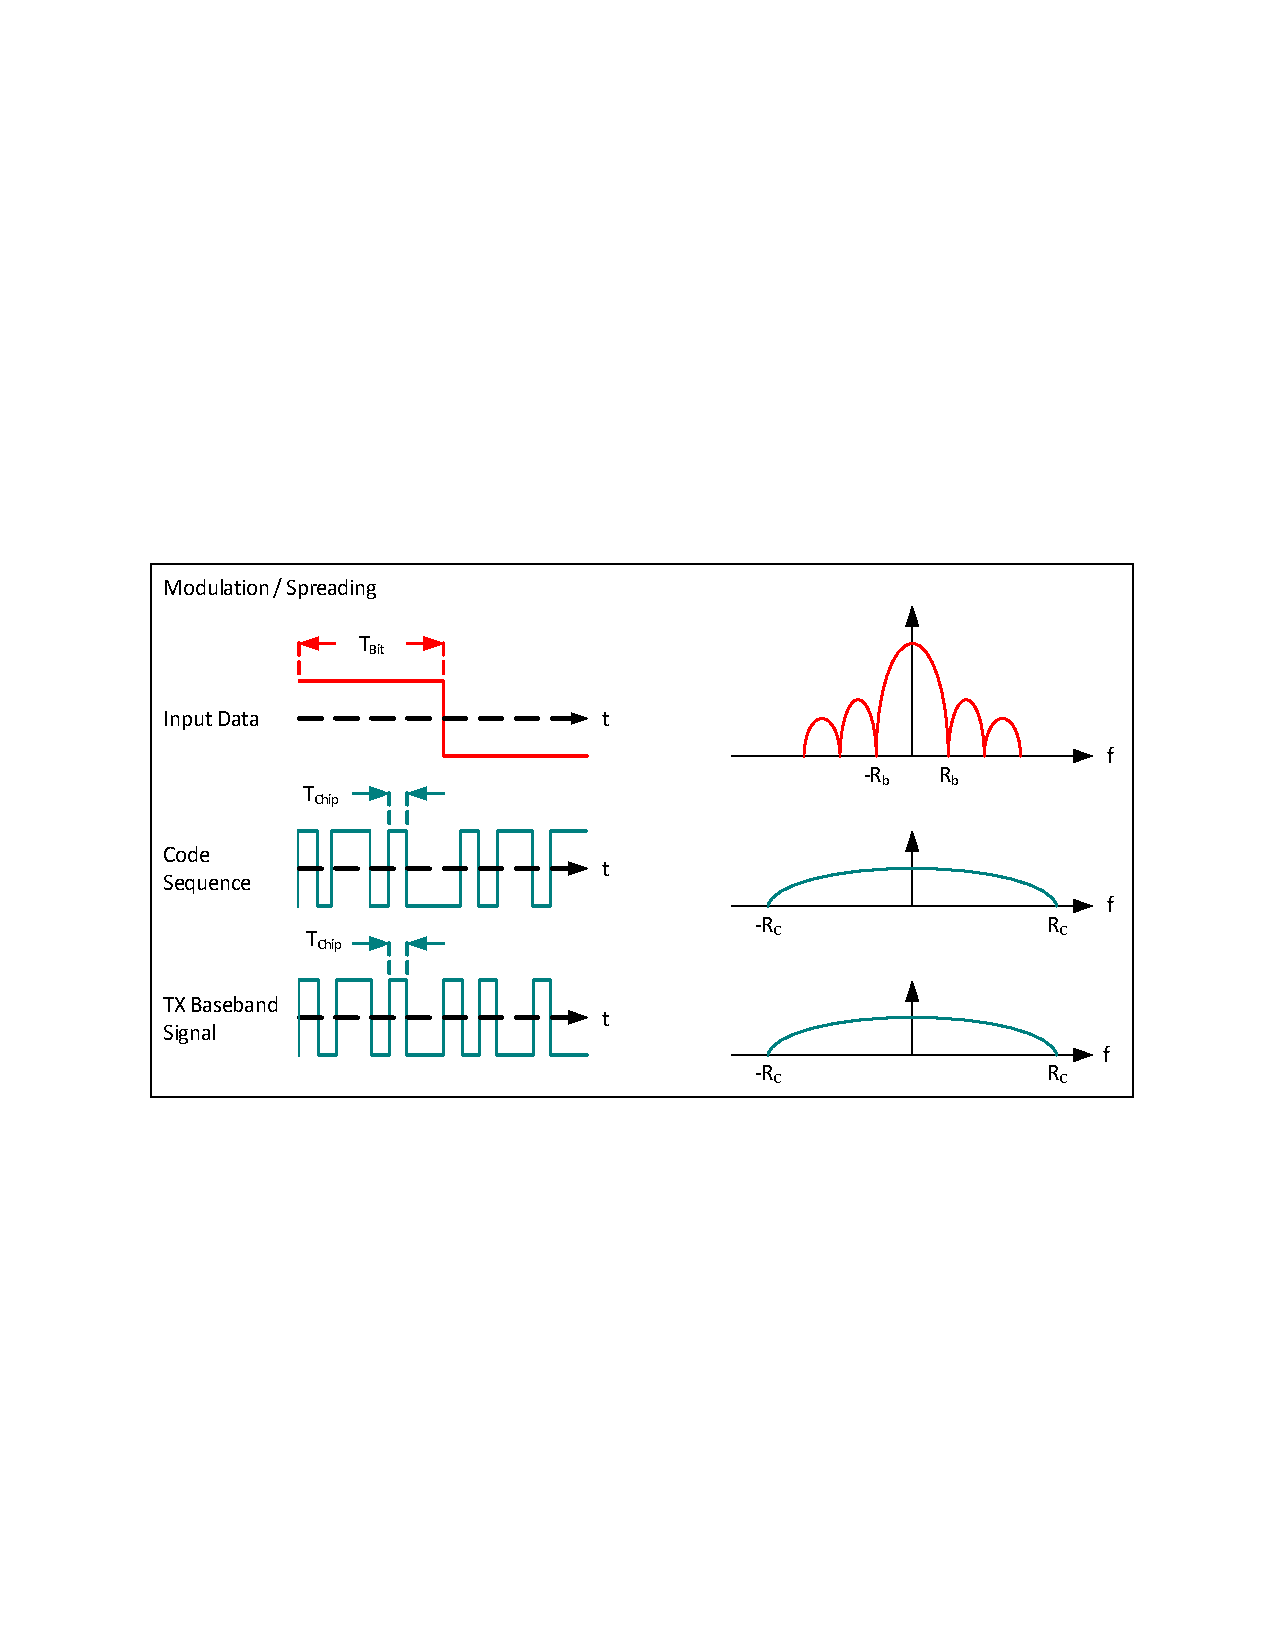
\includegraphics[width=0.8\linewidth]{./img/21.pdf}
			\caption{Kỹ thuật trải phổ sử dụng chuỗi mã trải phổ}
			\label{fig:fig21}
	\end{figure}
	
	\begin{figure}[h!] % hinh 22
			\centering
			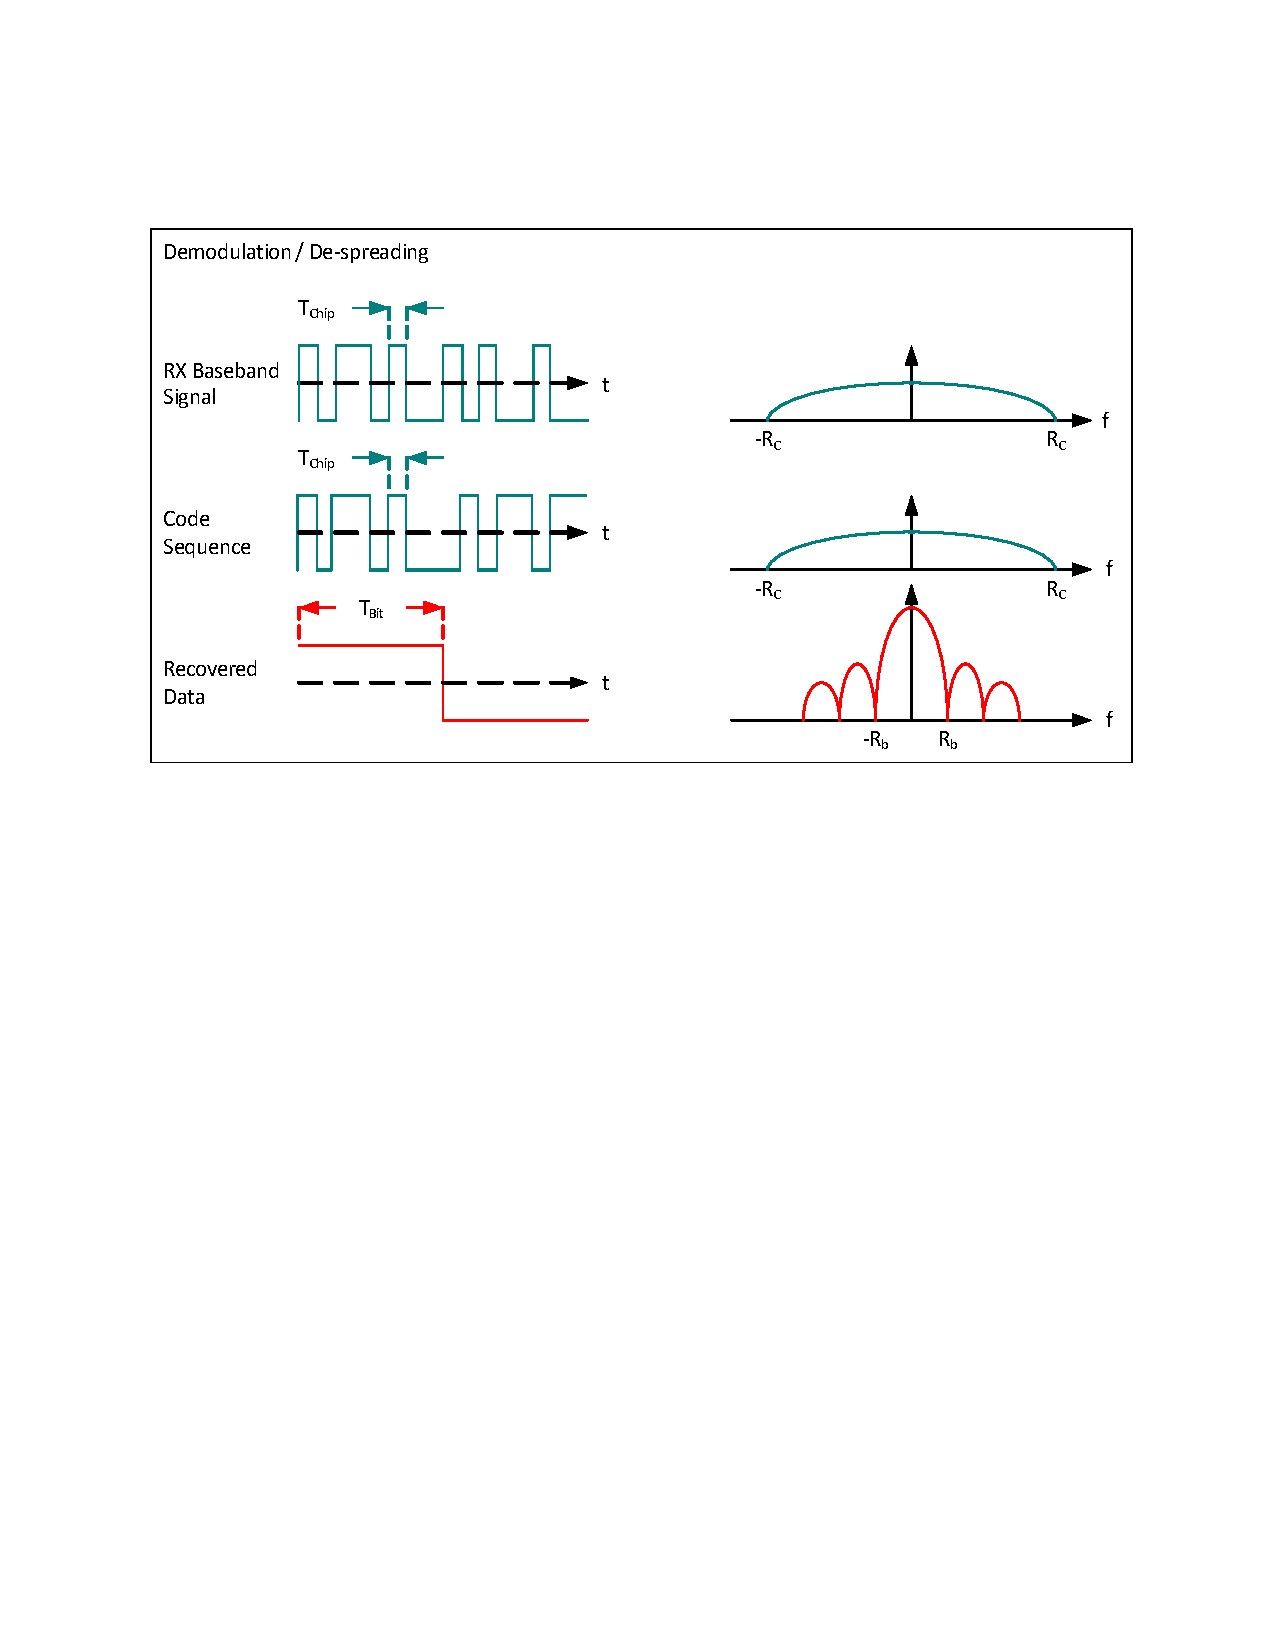
\includegraphics[width=0.8\linewidth]{./img/22.pdf}
			\caption{Sơ đồ giải trải phổ}}
			\label{fig:fig22}
	\end{figure}	
		
	Theo như công thức Shannon, khi tăng băng thông tín hiệu, ảnh hưởng của nhiễu có thể hạn chế tối thiểu. Kỹ thuật trải tín hiệu trên miền tần số được gọi là kỹ thuật trải phổ. Có nhiều loại  kỹ thuật trải phổ. Một trong những kỹ thuật cơ bản nhất là kỹ thuật trải phổ trực tiếp (DSSS), nó sử dụng một code có tần số lớn hơn với tín hiệu dữ liệu để trải phổ tần số của tín hiệu cần truyền. Mã code này được gọi là mã trải phổ hay chuỗi chip (chip sequence), nó được nhân với tín hiệu dữ liệu trước khi truyền đi. \par 
	Phía máy thu thực hiện tách tín hiệu dữ liệu bằng cách nhân với chuỗi trải phổ một lân nữa. \par
	Hệ số trải phổ của tín hiệu chip (chip signal) phụ thuộc và tỷ số chip rate và tốc độ dữ liệu yêu cầu (required data rate). Nó được gọi là processing gain ($G_p$), được tính theo công thức:
	\begin{equation}
	G_p = 10 \times log_{10}(\frac{R_c}{R_b})
	\end{equation}
Trong đó: 
\begin{itemize}
\item	$G_p$  = Processing gain (dB) 
\item	$R_c$  = chip rate (bps) 
\item	$R_b$  = bit rate yêu cầu (bps) 
\end{itemize}
Quá trình này không những tạo ra tín hiệu kháng lại nhiễu kênh truyền mà còn kháng được nhiễu từ các tín hiệu khác. Processing gain cho phép tái xây dựng lại tín hiệu ban đầu chính xác mặc dù SNR có thể âm. Bất kỳ can nhiễu nào cũng dễ dàng được lọc. \par
	Thách thức lớn nhất của việc triển khai DSSS cho các ứng dụng low-cost và công suất thấp là phải cần có một nguồn xung cực kỳ chính xác. Hơn thế nữa, yêu cầu chip codes dài hơn tốn thời gian giải trải phổ tại máy thu. Nó không những khiến cho máy thu trở nên phức tạp mà lại còn tăng thời gian xử lý ở máy thu. Phía thu  phải luôn ở trạng thái đồng bộ với máy phát, nó không thể đáp ứng được với một ứng dụng yêu cầu công suất thấp.
	\subsection{Chirp Spread-Spectrum}
	\begin{figure}[h!] % hinh 23
			\centering
			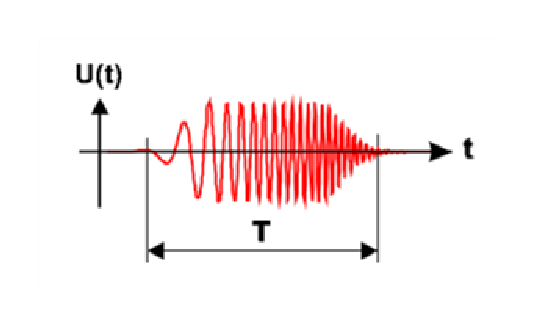
\includegraphics[width=0.5\linewidth]{./img/23.pdf}
			\caption{Up-chirp trong miền thời gian}
			\label{fig:fig23}
	\end{figure}
	
	\begin{figure}[h!] % hinh 24
			\centering
			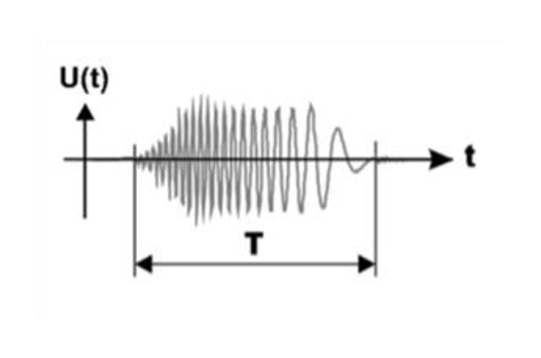
\includegraphics[width=0.5\linewidth]{./img/24.pdf}
			\caption{Down-chirp trong miền thời gian}
			\label{fig:fig24}
	\end{figure}
Một chirp là một tín hiệu hình sin tăng dần hoặc giảm dần của tần số theo thời gian. Nó dựa trên một tín hiệu chirp tự nhiên cho trải phổ băng thông của tín hiệu gửi. Một chirp tăng dần tần số được gọi là up-chirp được minh hoạ ở hình \ref{fig:fig23}. \par
Một chirp mà tần số giảm dần được gọi là down-chip, được mình hoạ ở hình \ref{fig:fig24}. \par 
Up-chirp là một chirp có giá trị dương còn down-chirp có giá trị âm. Sự thay đổi tần số có thể là tuyến tính hoặc theo hàm số mũ. Băng thông của một tín hiệu chirp có sự khác biệt giữa tần số đầu tiên và tần số kết thúc. 

\subsubsection{Nén xung (Pulse Compression)}
	\begin{figure}[h!] % hinh 25
			\centering
			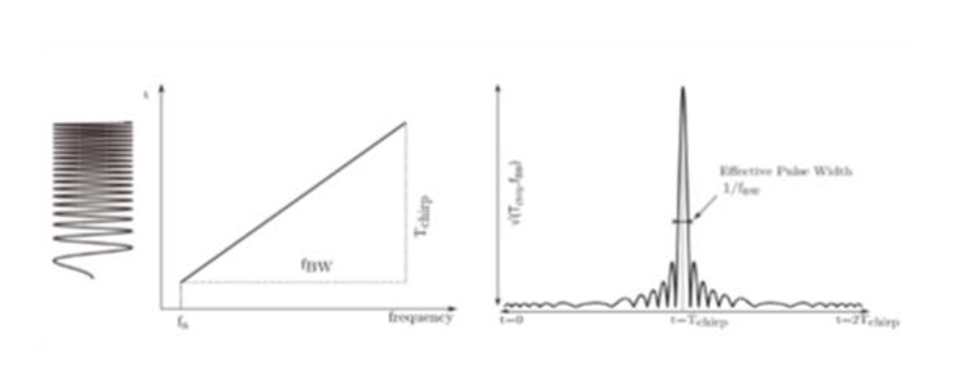
\includegraphics[width=0.8\linewidth]{./img/25.pdf}
			\caption{Xung chirp và kết quả xung sau khi nén}
			\label{fig:fig25}
	\end{figure}
		\begin{figure}[h!] % hinh 26
			\centering
			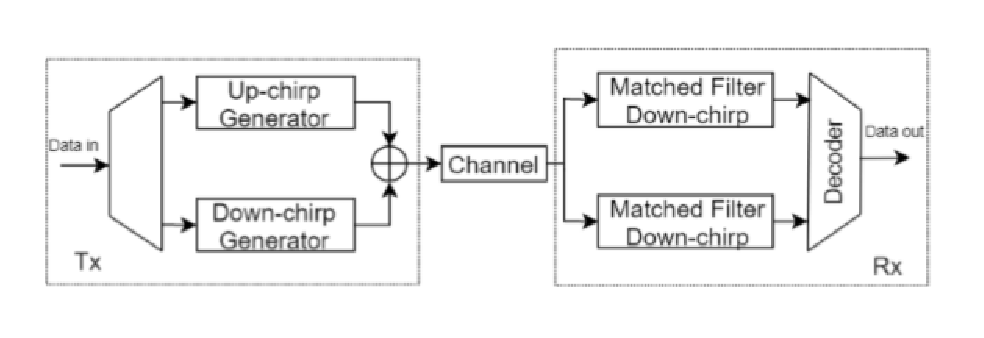
\includegraphics[width=0.8\linewidth]{./img/26.pdf}
			\caption{Xung chirp và kết quả xung sau khi nén}
			\label{fig:fig26}
	\end{figure}
Nén xung là một quá trình mà một xung có chu kỳ dài với công suất đỉnh thấp được biến đổi thành một xung có công suất đỉnh lớn và có chu kỳ ngắn. Chirps cho phép thực hiện nén xung rất thẳng bằng tương quan sử dụng một \textit{matched filter}. Đầu ra của sự tương quan với một \textit{matched filter} là một xung kết hợp  công suất của xung chirp trên chu kỳ hiện tại của nó (minh hoạ hình \ref{fig:fig25}). Kết quả là cho một processing gain lớn và \textit{distance resolution}. \par 

Hình \ref{fig:fig26} mô tả các khối chức năng của hệ thống CSS. Dữ liệu được điều chế sử dụng up và down chíp tại máy thu và giải điều chế sử dụng bộ tương quan + matched filter cho nén xung. Nhận lại được các xung nhọn có năng lượng cao dễ dàng cho việc giải mã. \par 
Đặc tính quan trọng của CSS là khoảng data rate rất lớn. Chirp dựa trên trải phổ có thể dùng để trải tín hiệu cả với miền thời gian và tần số.

\subsubsection{	Trải tần số (Frequency Spreading)}
Như giải thích ở trên, trải băng thông tín hiệu có thể làm giảm ảnh hưởng của nhiễu kênh truyền và làm cho tín hiệu miễn nhiễm với can nhiễu. Sử dụng xung chirp của băng thông cao hơn, băng thông tín hiệu có thể lớn hơn so với yêu cầu.
\subsubsection{	Trải thời gian (Time Spreading)}

Băng thông của tín hiệu chirp chỉ phụ thuộc vào tần số bắt đầu và tấn số kết thúc của chirp, data rate của kỹ thuật điều chế chirp có thể tăng hoặc giảm phụ thuộc vào băng thông. Nên có thể tự do lựa chọn băng thông và tốc độ dữ liệu của tín hiệu mong muốn và điều chỉnh BT product như yêu cầu. Nó có kết quả với tín hiện robust và high BT product. \par 
	Hệ thống CSS có nhiều sự khác nhau tuỳ thuộc vào yêu cầu của ứng dụng. Các đặc điểm nổi bật khác bao gồm: interference robustness, kháng đa đường, công suất thấp, trễ thấp và CSS không cần đồng bộ. Với những đặc điểm trên CSS đã được phát triển trong chuẩn IEEE 802.15.4. 
	
	\subsection{LoRa Chirp Spread-Spectrum}
	Kỹ thuật điều chế tại LoRa PHY [4] được phát triển dựa trên CSS truyền thống, kết hợp thêm các đặc điểm của hệ thống DSSS. Tín hiệu LoRa được điều chế sử dụng một tín hiệu chirp tần số biến đổi liên tục. Loại bỏ sự cần thiết có một nguồn xung đồng hồ chính xác và sự đồng bộ tại phía thu. Cả offset tần số và offset thời gian đề tương đương ở cả phía phát và phía thu. Điều này làm cho PHY đơn giản hơn và có khả năng hoạt động yêu cầu công suất thấp và robust communication link. \par  
	Băng thông của tín hiệu chirp sinh ra cho trải phổ là tương tương với tín hiệu.
Bit-rate của điều chế LoRa được định nghĩa bởi công thức:
	\begin{equation}
	R_b = SF \times \frac{1}{T_s}
	\end{equation}
	Trong đó: 
\begin{itemize}
\item	$R_b$  là bit-rate (bps) 
\item	$SF$ là hệ số trải phổ từ 7 – 12 
\item	$T_s$ là chu kỳ ký tự (s) 
\end{itemize}
	Chu kỳ ký tự được định nghĩa:
	\begin{equation}
	T_s = \frac{2^{SF}}{BW}
	\end{equation}
	Trong đó, BW là băng thông của tín hiệu điều chế (Hz). Theo sự tương quan ở trên, bit-rate và chu kỳ ký tự tỷ lệ nghịch với nhau và tỷ lệ thuận với hệ số trải phổ. \par 
Chip rate của kỹ thuật điều chế LoRa được định nghĩa:
\begin{equation}
R_c = R_s \times 2^{SF}
\end{equation}
Trong đó: 
\begin{itemize}
\item	$R_c$  là chip rate (chips per second) 
\item	$R_s$  là symbol rate (symbol per second) 
\end{itemize}
	Symbol rate được định nghĩa như sau: 
	\begin{equation}
	R_s = \frac{1}{T_s} = \frac{BW}{2^{SF}}
	\end{equation}
	Nên:
	\begin{equation}
	R_c = \frac{BW}{2^{SF}}\times 2^{SF}
	\end{equation}
	Vậy nên LoRa gửi một chip trên một giây trên một Hertz. Hơn thế nữa, mã sửa sai có chiều dài biến đổi cũng được sử dụng nhằm tăng robustness. Kết quả data-rate của kỹ thuật điều chế LoRa như sau:
	\begin{equation}
	R_b = SF \times \frac{\frac{4}{4+CR}}{\frac{2^{SF}}{BW}}
	\end{equation}
	Trong đó:
\begin{itemize}
\item	$CR$ là coding rate khoảng từ 1 đến 4
\item	$SF$ là hệ số trải phổ khoảng từ 7 – 12
\item	$BW$ là băng thông tín hiệu, thường dùng 125, 250 và 500 kHz.
\end{itemize}


\subsection{Các đặc điểm nổi bật}

\subsubsection{	Tích tần số - thời gian cao}
Điều chế LoRa có thể tạo nên tích tần số thời gian (bandwidth-time product) lớn hơn 1 [4]. Khi có sự kết hợp giữa báo hiệu không đồng bộ, nó khiến tín hiệu LoRa tốt hơn về cả băng tần cũng như băng can nhiễu. Điều chế LoRa có thể xây dựng sự chọn lọc kênh lên đến tới 90 dB và in-band rejection lên tới 20 dB.
\subsubsection{	Khả năng mở rộng của băng thông}
Điều chế LoRa có khả năng đáp ứng cả ứng dụng băng rộng và băng hẹp do vì sự khả năng mở rộng vốn có (inherent scability) của tần số và băng thông. Module LoRa có thể dễ dàng cấu hình để phù hợp với các loại ứng dụng bằng cách thay đổi giá trị (SF, BW, công suất phát) các thanh ghi cấu hình.
\subsubsection{	Mức tiêu thụ năng lượng thấp}
LoRa Modulation thừa kế đặc tính đường bao không đổi (constant envelope) của kỹ thuật điều chế FSK, do đó nó có khả năng sử dụng ít năng lượng và hiệu quả ở trạng thái khuếch đại công suất. Hơn thế nữa, processing gain của trải phổ chirp cũng cho phép công suất đầu ra của bộ phát được giảm xuống mà không làm giảm quỹ đường truyền (link budget).
\subsubsection{	Multipath Robustness}
LoRa có khả năng chống lại hiệu ứng đa đường và hiệu ứng fading ở trong môi trường đô thị.
\subsubsection{	Long Range}
LoRa có khoảng cách truyền thông lớn so với các kỹ thuật như FSK ở cùng mức năng lượng. Khi kết hợp các thuộc tính robustness đã trên trên, quỹ đường truyền (link budget) của LoRa có thể dịch 4 lần tăng cường ở khoảng cách.
\subsubsection{	Kháng lại hiệu ứng Doppler}
LoRa có khả năng kháng hiệu ứng Doppler. Nó khiến cho LoRa có thể ứng dụng trong các ứng dụng có tính di động [4].
\subsubsection{	Tăng cường dung lượng mạng}
Nhiều tín hiệu trải phổ có thể được truyền đồng thời thông qua cùng một kênh vì LoRa sử dụng các hệ số trải phổ trực giao. Tín hiệu sử dụng các hệ số trải phổ khác sẽ được lọc như một tín hiệu nhiễu tại máy thu.
\subsubsection{	Đặc điểm về định vị}
LoRa có khả năng phân biệt được giữa lỗi thời gian và tần số, nó cho phép có thể ứng dụng trong các ứng dụng định vị và khoảng cách.

\subsection{Các tham số kỹ thuật chính}
Dưới đây là một số tham số đặc trưng, quan trọng nhất của tầng vật lý LoRa:
\begin{itemize}
\item Tần số sóng mang (carrier frequency- CF): biểu diễn tần số trung tâm của dải tần số truyền dẫn tín hiệu. Tất cả gồm ba dải tần số (433 MHz, 868MHz, 915MHz) được đặc tả trong datasheet SX1278 Semtech,
\item Băng thông (BW): Là khoảng tần số có khả năng cho tín hiệu truyền qua. Semtech SX1276 đưa ra băng tần từ 7.8kHz đến 500kHz. Băng thông lớn cho phép truyền dữ liệu với datarate cao, thời gian trong không gian thấp (time on air) nhưng độ nhạy thu thấp như là kết quả của nhiễu. Những giá trị băng thông hay được sử dụng trong truyền thông LoRa: 125, 250 và 500 kHz,
\item Hệ số trải phổ (SF): biểu thị cho tỷ số chirp (chirp rate) sử dụng để truyền dữ liệu thông qua băng thông khả dụng. Với một SF, thì ta có 2SF chips/symbol. SF thường dùng từ SF6 đến SF12. Với SF12 thì ta có độ nhạy thu và khoảng cách truyền phát là lớn nhất, nhưng tốc độ truyền thấp nhất (Hệ số trải phổ tỷ lệ thuận với khoảng cách truyền thông và tỷ lệ nghịch với tốc độ data rate),
\item Coding Rate (CR): được sử dụng trong công nghệ LoRa là một tỷ số sửa lỗi trước (Forward Error Correction FEC rate). Nó cho phép khôi phục lại các bit thông tin bị lỗi do tạp âm. Tỷ số CR cao thì khả năng sửa lỗi cũng tăng nhưng thời gian ngoài không gian (ToA) cũng tăng. Với LoRa, CR có thể là 4/5, 4/6, 4/7 hoặc 4/8,
\item Độ nhạy thu $\rho$ (dBm) được định nghĩa bởi Semtech: $\rho (dBm) = −174 + logBW + NF + SNR$. Trong đó -174dB là nhiễu theo lý thuyết, BW băng thông kênh truyền, NF là hệ số tạp âm máy thu (tùy vào phần cứng, với SX1276, SX1272 NF = 6 dB), SNR là tỷ số công suất tín hiệu trên công suất nhiễu.

\end{itemize}

\subsection{Thời gian truyền}
Thời gian truyền của bản tin LoRa phụ thuộc vào các tham số chính như $BW$, $CR$, $SF$. Sự kết hợp của ba tham số sẽ cho kết quả thời gian truyền của bản tin có sự khác nhau.
Như công thức tính symbol-rate $T_s = \frac{1}{R_s}$, tổng thời gian truyền 1 bản tin của LoRa còn phụ thuộc vào trường mào đầu. Chu kỳ cho một phiên truyền trường mào đầu như sau:
\begin{equation}
T_{preamable} = (n_{preamable} + 4.25) \times T_s
\end{equation}
Trong đó:
\begin{itemize}
\item $n_{preamable}$ là chiều dài trường mào đầu (10 - 65540)
\item $T_{preamble}$ là thời gian truyền trường mào đầu
\item $T_s$ là symbol rate của một preamble
\end{itemize}
Tương tự, thời gian truyền của payload phụ thuộc vào số lượng ký tự trong payload. Chiều dài ký tự của payload với explicit header được tính như sau:
\begin{equation}
{{n}_{payload}}=8+max(cell\frac{(2P+4CRC-SF+7)}{(SF-2D)}(CR+4),0)
\end{equation}
Và cho implicit header như sau:
\begin{equation}
{{n}_{payload}}=8+max(cell\frac{(2P+4CRC-SF+2)}{(SF-2D)}(CR+4),0)
\end{equation}
Trong đó:
\begin{itemize}
\item	SF là hệ số trải phổ được chọn
\item	D = 1 khi tối ưu data rate được bật và ngược lại
\item	CR là coding rate (tỷ số mã hoá)
\item	CRC = 1 khi CRC được chọn
\item	P là số byte của payload (1 - 255)
\end{itemize}
Kết quả chu kỳ truyền dần của payload như sau:
\begin{equation}
T_{payload} = n_{payload} \times T_s
\end{equation}
Tổng thời gian truyền tính:
\begin{equation}
T_{packet} = T_{payload} + T_{preamble}
\end{equation}

\section{Giao thức chuẩn mở LoRaWAN}
Trong mục này em trình bày những đặc điểm cốt lõi của chuẩn mở LoRaWAN. Bao gồm các điểm chính như kiến trúc hệ thống, mô hình chồng giao thức, các lớp thiết bị được phân loại theo chuẩn LoRaWAN, cơ chế điều khiển đa truy nhập lớp MAC, các loại bản tin, tiến trình thực hiện trong mạng LoRaWAN Alliance. Tất cả sẽ được trình bày chi tiết lần lượt ở các mục phía dưới.
\subsection{Đặc tả kỹ thuật}

\subsubsection{Kiến trúc hệ thống}
	\begin{figure}[h!] % hinh 27
			\centering
			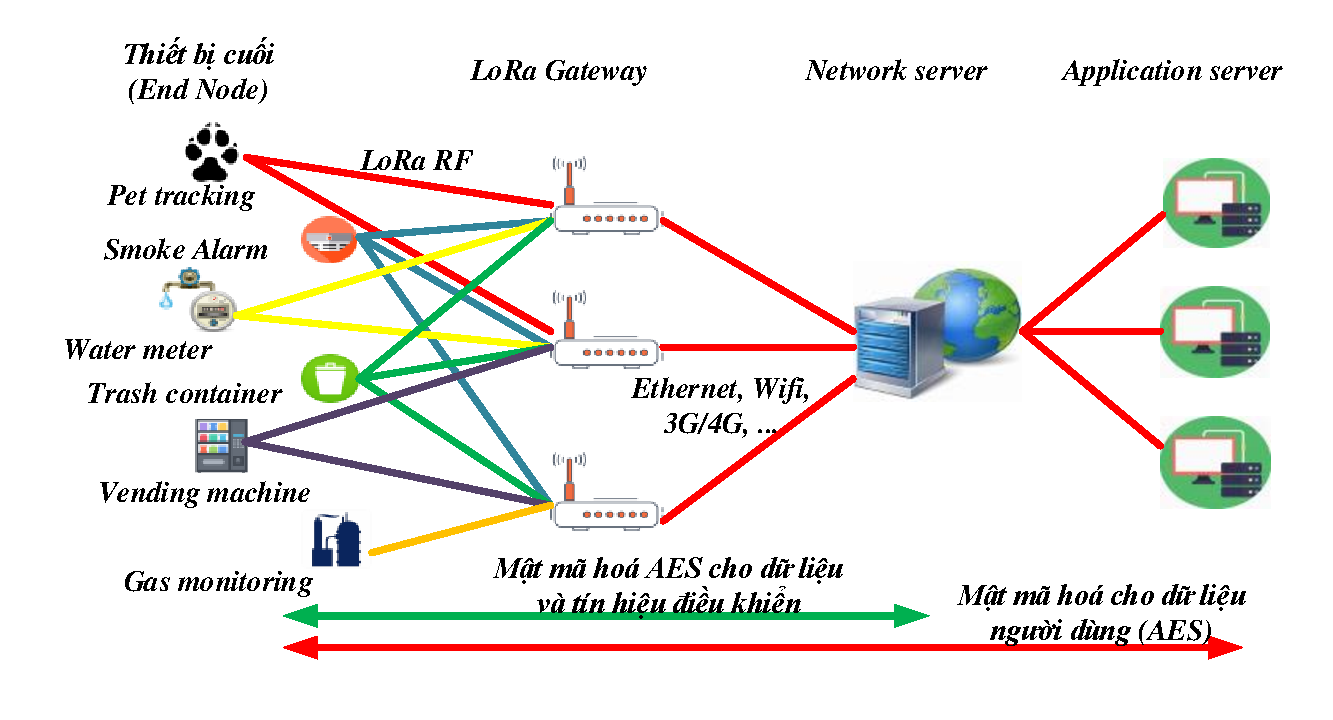
\includegraphics[width=1\linewidth]{./img/27.pdf}
			\caption{Kiến trúc hệ thống mạng LoRaWAN}
			\label{fig:fig27}
	\end{figure}
	\begin{figure}[h!] % hinh 28
			\centering
			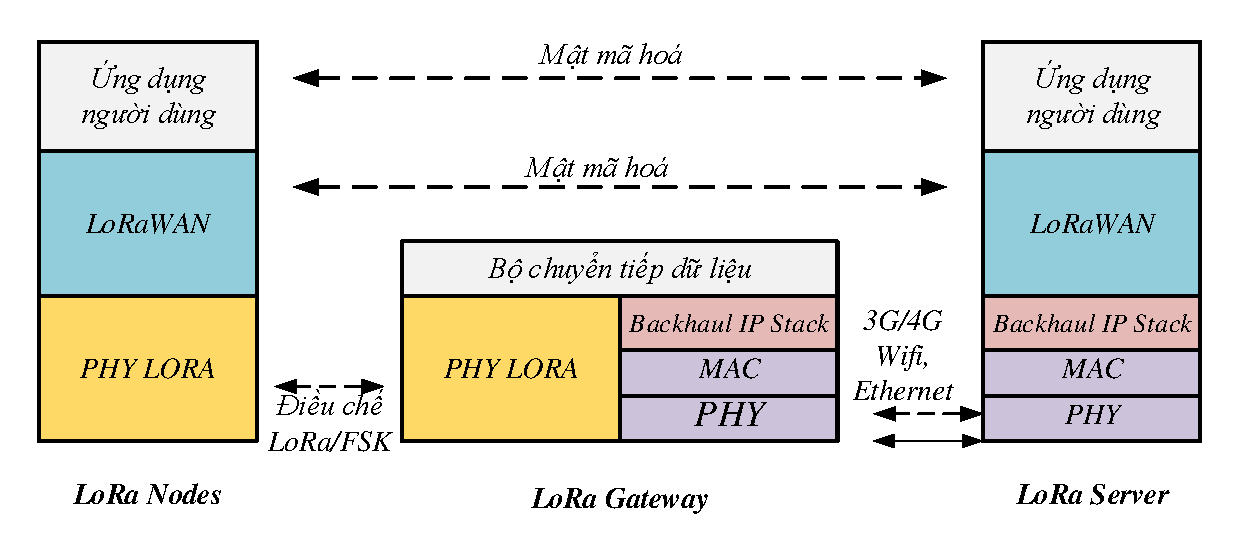
\includegraphics[width=1\linewidth]{./img/28.pdf}
			\caption{LoRaWAN Stack Protocol}
			\label{fig:fig28}
	\end{figure}	
	
LoRaWAN Alliance là một chuẩn mở truyền thông không dây sử dụng tầng vật lý là công nghệ điều chế LoRa, được thiết kế để phù hợp với cự ly tryền thông lớn nhưng mức tiêu thụ năng lượng thấp và được dựa trên hệ thống truyền thông Radio đơn chặng. Một mạng LoRaWAN được thiết kế theo đồ hình hình sao của các hình sao (star of stars topology) được cấu thành từ 3 phần tử cơ bản: thiết bị cuối (vd: sensor node), gateways, một máy chủ mạng trung tâm đôi khi có thể thêm một server ứng dụng Hình \ref{fig:fig27}.
\begin{itemize}
\item	Thiết bị đầu cuối, thường là các nút mạng cảm biến, thu thập dữ liệu vật lý từ các hệ cảm biến. Thiết bị đầu cuối này có tích hợp module truyền thông LoRa (thường là các dòng chip thu phát LoRa của Semtech) có chức năng truyền thông với gateways thông qua công nghệ điều chế LoRa.
\item	Gateways điều phối các khung thông tin từ thiết bị đầu cuối tới server mạng sử dụng một giao diện Backhaul với thông lượng lớn, thường là Ethernet, WiFi, 3G/4G hoặc vệ tinh. Một bản tin từ một thiết bị đầu cuối phát quảng bằng LoRa có thể nhận được từ nhiều Gateway. Tất cả các bản tin này đều được chuyển tiếp về phân hệ backend. Tuy nhiên, tại NS (Network Server) chuẩn LoRaWAN đã đưa ra cơ chế xoá những bản tin trùng lặp.
\item	Server mạng giải mã các gói tin gởi bởi thiết bị đầu cuối, thực hiện kiểm tra mã hóa và Data-rate đáp ứng (apdaptive data rate) và tạo ra các gói tin phản hồi tới thiết bị đầu cuối.
\item	Mỗi ứng dụng nhận dữ liệu từ server. Nó có thể giải mã gói tin được bảo mật và dùng thông tin đó cho các chức năng của ứng dụng.
\end{itemize}
Liên kết truyền thông lớn, số lượng anten (trạm gateway), và thời gian sử dụng pin của thiết bị đầu cuối được cải thiện nhờ kiến trúc mạng hình sao. Truyền thông với tốc độ dữ liệu (Data rate) khác nhau không có tạp âm, tốc độ dữ liệu nằm trong khoảng 300 bps tới 5 kbps, băng thông 125 kHz. \par 
	Hình \ref{fig:fig28} minh hoạ chồng giao thức (protocol stack) của giao thức LoRaWAN. Ở phía LoRa Nodes, có 3 tầng giao thức được cài đặt bao gồm: (i) tầng ứng dụng; (ii) tầng MAC; (iii) tầng vật lý. (i) Về tầng ứng dụng, tầng này được cài đặt trên LoRa Nodes có thể triển khai các ứng dụng như quan trắc các tham số môi trường, ví dụ, nhiệt độ, độ ẩm, cảm biến gas, khói trong một toà nhà. Dữ liệu đo được sẽ được xử lý và đóng gói gửi xuống tầng MAC (LoRaWAN), tầng này được cài đặt các thành phần tuân thủ theo đặc tả kỹ thuật của chuẩn LoRaWAN [5], bao gồm các cơ chế điều khiển đa truy nhập, các loại bản tin điều khiển MAC, các bản tin kiểm tra thông tin điều khiển. Sau khi, được đóng gói theo chuẩn LoRaWAN, toàn bộ khung sẽ được đẩy xuống tầng vật lý. Tại tầng vật lý, dữ liệu đóng gói thêm header của LoRa Module rồi được tiến hành điều chế trước khi gửi ra antenna. Quá trình nhận dữ liệu được thực hiện ngược lại.\par
	Tiếp theo là chồng giao thức được cài đặt trên LoRa Gateway. Một bộ chuyển tiếp gói được cài đặt, nó điều khiển giao thức lớp vật lý LoRa Gateway (Sử dụng module LoRa dành chuyên cho gateway – có khả năng nhận và xử lý đồng thời nhiều bản tin) nhằm nhận/phát các bản tin LoRa RF. Dữ liệu được cộng thêm siêu dữ liệu (metadata) là các thông tin bổ sung về tình trạng của hệ thống rồi chuyển đổi thành IP thông qua Ethernet, Wifi hoặc IP thông qua mạng thông tin di động. Dữ liệu được đẩy qua các tầng giao thức Backhaul IP Stack, MAC, PHY tuỳ thuộc loại công nghệ được lựa chọn. \par
	Tại LoRa Server, một chồng giao thức TCP/IP cũng được tích hợp ở đáy để nhận các bản tin UDP mà gateway gửi lên, dữ liệu sau khi được tách header TCP/IP được đưa đến bộ giao thức LoRaWAN, tương ứng với của LoRa Nodes để tách dữ liệu. Cuối cùng, gửi lên đến tầng ứng dụng, trọn đủ giao thức từ tiến trình đến tiến trình.
	
\subsubsection{LoRaWAN Classes}
	\begin{figure}[h!] % hinh 29
			\centering
			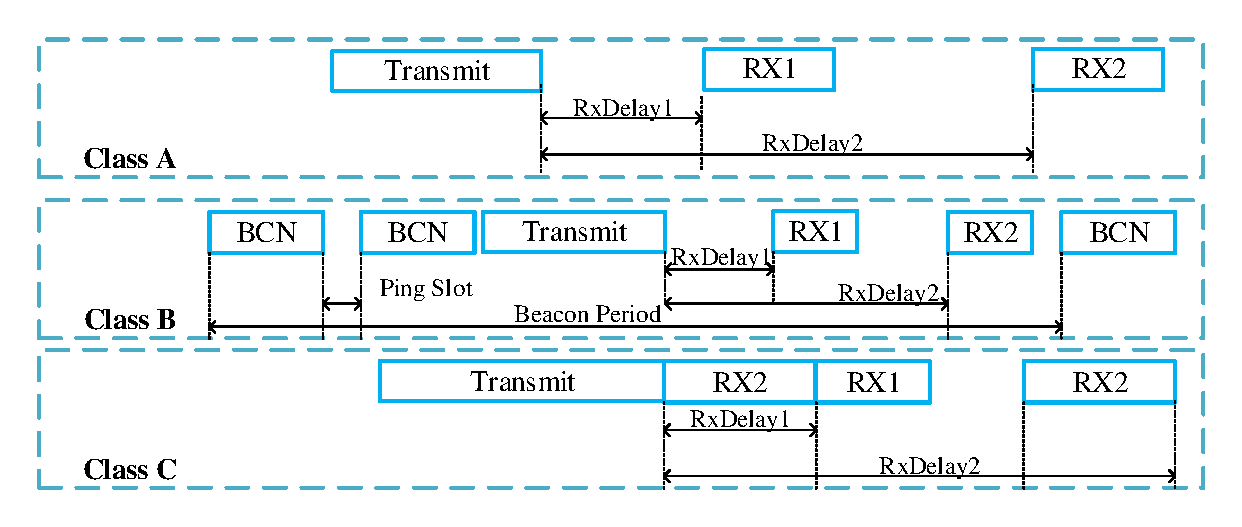
\includegraphics[width=\linewidth]{./img/29.pdf}
			\caption{Các lớp theo chuẩn LoRaWAN Alliance}
			\label{fig:fig29}
	\end{figure}
LoRaWAN định nghĩa ba lớp chức năng: Class A, class B và class C (Hình \ref{fig:fig29}):
\begin{itemize}
\item	Class A (song phương): class A được thực thi bởi tất cả các thiết bị LoRaWAN, nó được biết đến là cơ bản của LoRaWAN. Class A cho phép truyền thông song phương giữa một thiết bị đầu cuối và server mạng, nó có một cửa số truyền dần uplink (TX window - node tới server) theo bởi 2 cửa sổ truyền dẫn downlink nhỏ hơn (2 RX window). Các khe truyền dẫn được lập lich theo cơ chế điều khiển đa truy nhập ngẫu nhiên cơ bản là ALOHA. Mức tiêu thụ năng lượng ở lớp A là lớn nhất, trễ cũng lớn nhất,
\item	Class B được thiết kế dựa trên lớp A, tuy nhiên nó được hỗ trợ thêm cơ chế lập lịch truyền dẫn đường xuống (additional scheduled downlink transmission). Mức tiêu thụ năng lượng là trung bình (cao hơn classA và thấp hơn classC),
\item	Class C: Thiết bị mở cửa số nhận liên tục, tương tự như thuật toán cửa sổ trượt. Nó có mức tiêu thụ năng lượng cao nhưng trễ truyền lan là nhỏ nhất. Theo đặc tả kỹ thuật của Alliance thì các thiết bị phải thực hiện tất cả chức năng của lớp A, còn lớp B, C là các tùy chọn cho các ứng dụng phức tạp hơn.

\end{itemize}

\subsubsection{Cấu trúc bản tin}
	\begin{figure}[h!] % hinh 210
			\centering
			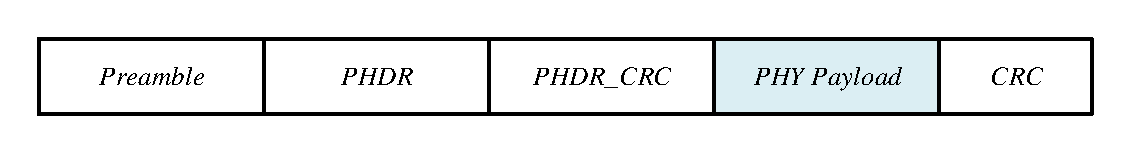
\includegraphics[width=0.8\linewidth]{./img/210.pdf}
			\caption{Cấu trúc khung truyền tầng vậy lý LoRa}
			\label{fig:fig210}
	\end{figure}
		\begin{figure}[h!] % hinh 211
			\centering
			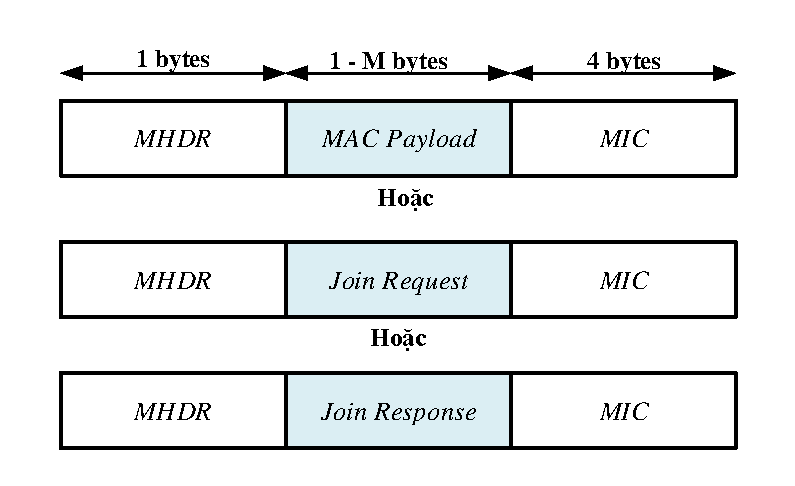
\includegraphics[width=0.7\linewidth]{./img/211.pdf}
			\caption{Cấu trúc PHY LORA Payload}
			\label{fig:fig211}
	\end{figure}
		\begin{figure}[h!] % hinh 212
			\centering
			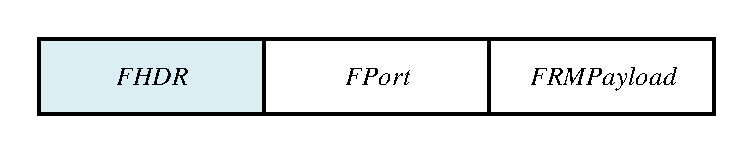
\includegraphics[width=0.7\linewidth]{./img/212.pdf}
			\caption{Cấu trúc khung MAC Payload}
			\label{fig:fig212}
	\end{figure}
		\begin{figure}[h!] % hinh 213
			\centering
			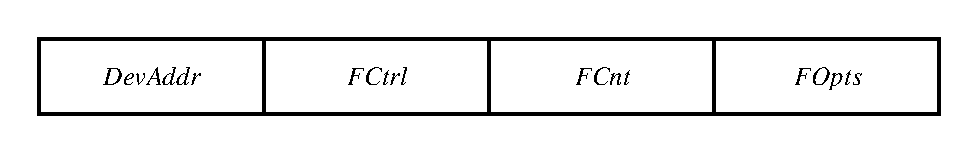
\includegraphics[width=0.8\linewidth]{./img/213.pdf}
			\caption{Cấu trúc khung FHDR}
			\label{fig:fig213}
	\end{figure}
	Hình \ref{fig:fig210} minh hoạ cấu trúc bản tin được gửi đi tại tầng vật lý LoRa, gồm các trường đầu tiên là trường mào đầu (preamble), tiếp đến là PHY Header và một trường CRC cho PHY Header. Tiếp đến là phần payload của bản tin tầng vật lý, cuối cùng là trường CRC cho toàn bộ bản tin. \par 
	Lên đến giao thức tầng MAC, nội dung PHY Payload có thể là một trong 3 cấu trúc như minh hoạ Hình \ref{fig:fig211}, bao gồm một tường MAC Header, một trường MIC để kiểm tra tính toàn vẹn của dữ liệu. Trường ở giữa có thể là MAC Payload, yêu cầu tham gia mạng (Join Request) hoặc phản hồi yêu cầu tham gia mạng (Join Respone). Khi trường dữ liệu ở giữa là Join Request hoặc Join Response thì đó bản tin dùng trong quá trình thực hiện kích hoạt thiết bị cuối – cuối. Còn trong trường hợp truyền dữ liệu hoặc trao đổi các bản tin điều khiển MAC thì trường đó là MAC Payload.  \par 
	Với MAC payload (Hình \ref{fig:fig212}) thì khung gồm 3 trường là FHDR, FPort và FRMPayload, trương FRMPayload sẽ trực tiếp chứa dữ liệu người dùng khi trường FPort khác không. Trường hợp FPort bằng không, thì trường FRMPayload rỗng, bản tin khi này là bản tin điều khiển lớp MAC. Cụ thể hơn trong trường FHDR (Hình \ref{fig:fig213}) chứa 4 bytes là DevAddr, một trường điều khiển khung (FCtrl), một trường đếm khung (FCnt) và trường cuối cùng là FOpts là trường trực tiếp chứa mã của câu lệnh điều khiển MAC (MAC commands – cụ thể các câu lệnh MAC xem tại đặc tả chuẩn LoRaWAN [6]) 

\subsubsection{Các lệnh điều khiển MAC}

Về cơ bản, MAC command dùng để điều khiển khiển mạng, nó được dùng bởi LoRa Nodes tương tác với NS ở lớp MAC. Nó cung cấp các công cụ nhằm kiểm tra khi thiết bị Node có kết nối chính chính xác trong LoRaWAN. Một số câu lệnh MAC thường được trao đổi như DutyCycleReq, DevStatusReq, RXTimingSetupReq, … nhằm để kiểm tra trạng thái thiết bị, điều kiện kênh truyền, khe của sổ nhận,… Bởi vậy, MAC commands được trao đổi thông qua trường tuỳ chọn khung (Frame option field) hoặc trong FRMPayload. FRMPayload chứa Fport với giá trị bằng không nếu MAC commands được biểu diễn trong đó. Nhưng, trong khi dữ liệu được mã hoá thì đối với MAC command thì không được mật mã hoá. 
\subsection{Cơ chế kích hoạt các thiết bị (End-node, LoRa Nodes)}
		\begin{figure}[h!] % hinh 214
			\centering
			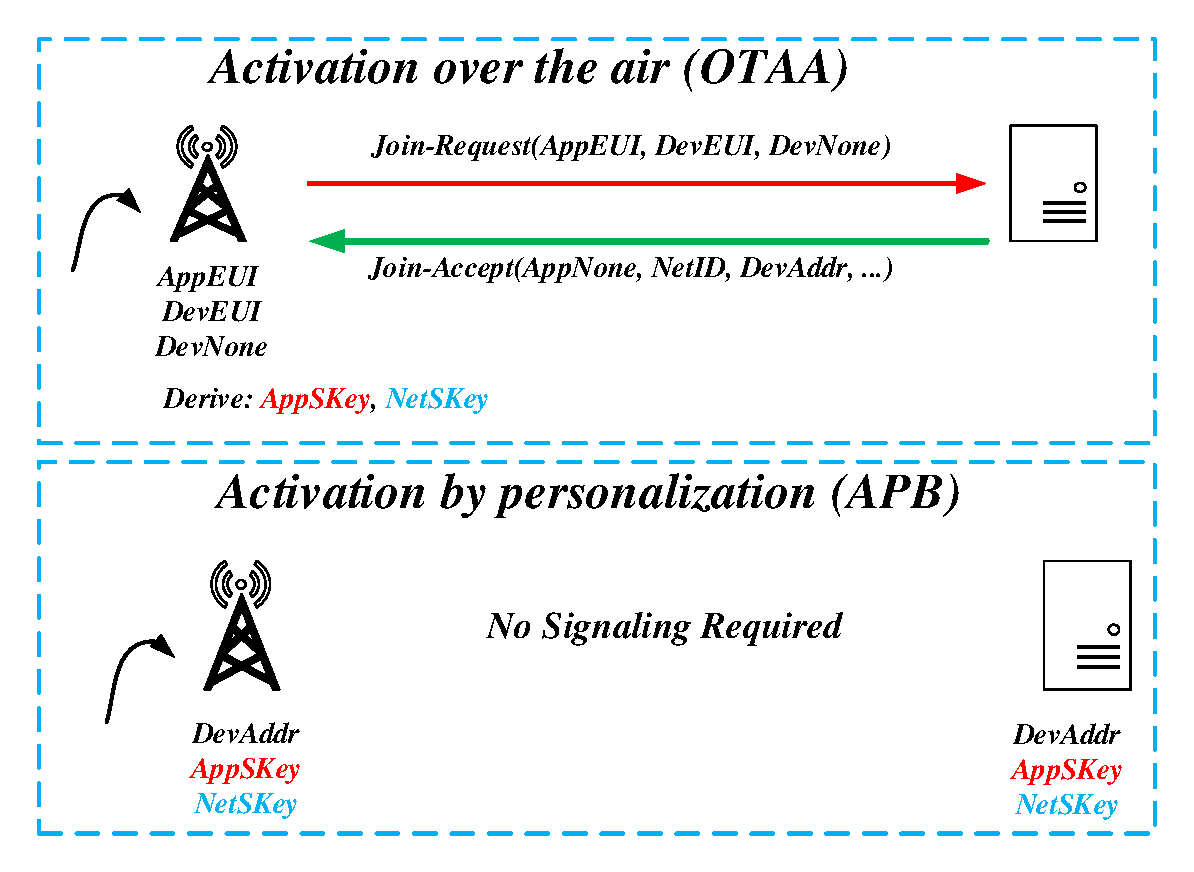
\includegraphics[width=\linewidth]{./img/214.pdf}
			\caption{Cơ chế kích hoạt LoRa Node}
			\label{fig:fig214}
	\end{figure}
Phiên bản mới nhất của chuẩn LoRaWAN là phiên bản v1.1 được công bố năm 2017, trong phạm vi đồ án này em thực hiện triển khai thực thi theo chuẩn cũ hơn là v1.0.3 (2016) nên các tên, chức năng các khoá được sử dụng cũng khác với phiên bản 1.1. Số lượng các khoá được lưu trên thiết bị giữa các phiên bản khác nhau, việc tạo ra các khoá trung gian và các quá trình tính toán bảo mật giữa các phiên bản cũng khau. Để hiểu chi tiết hãy xem các phiên bản chuẩn của Alliance cung cấp. \par 
	Hình \ref{fig:fig214} minh hoạ hai quá trình kích hoạt thiết bị của chuẩn LoRaWAN. Cơ chế đơn giản là cơ chế tự kích hoạt bằng tay. Với cơ chế này, một LoRa Nodes muốn tham gia mạng không phải trao đổi bản tin điều khiển với LoRa Server, mà sẽ cấu hình trực tiếp AppSKey, NetSKey trên LoRa App Server và LoRa Nodes. Sau đó, thiết bị sẽ gửi dữ liệu lên Server ngay. \par 
	Quá trình kích hoạt khác là quá trình kích hoạt tự động (Over The Air Activation), với quá trình này, thiết bị LoRa Nodes được cấu hình sẵn AppEUI, DevEUI là các mã định danh duy nhất. Trong quá trình này, LoRa Nodes và LoRa App Server sẽ trao đổi các bản tin Join Request và Join Response trước khi một LoRa Nodes chính thức tham gia mạng và gửi dữ liệu về ứng dụng. 

\subsubsection{Cơ chế bảo mật}
		\begin{figure}[h!] % hinh 215
			\centering
			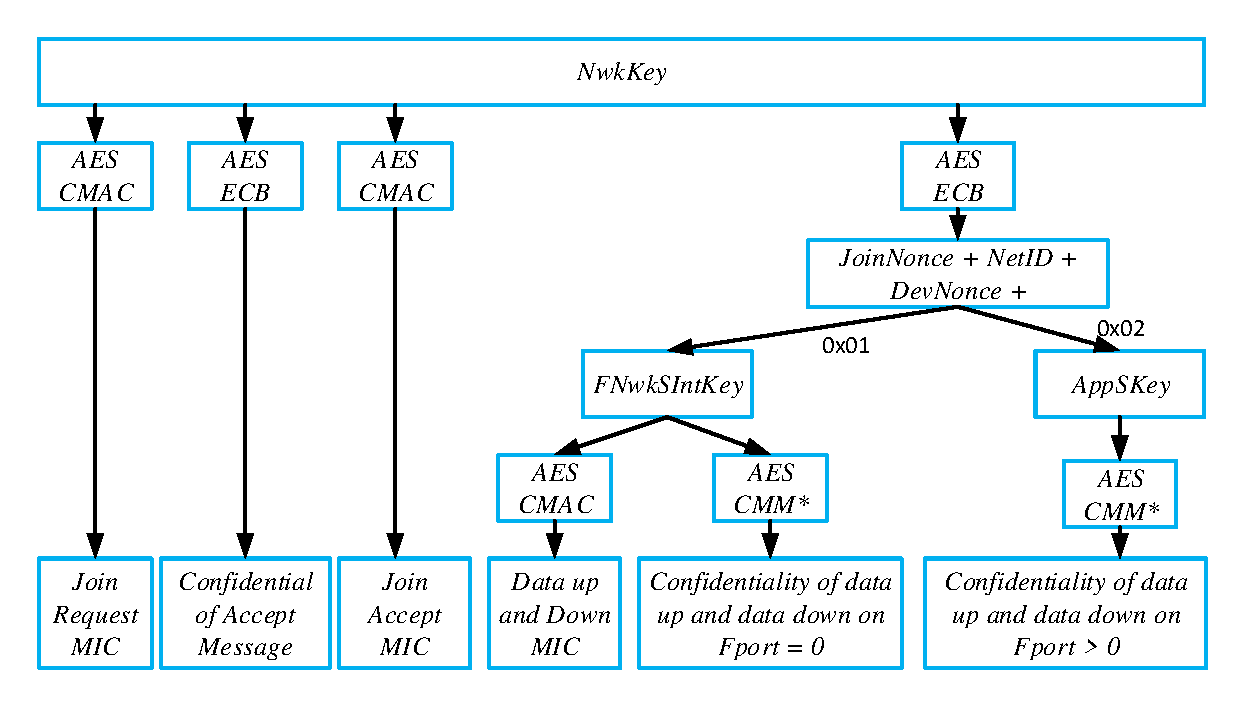
\includegraphics[width=\linewidth]{./img/215.pdf}
			\caption{Sơ đồ sinh khoá được sử dụng trong chuẩn LoRaWAN 1.0.3}
			\label{fig:fig215}
	\end{figure}
	Trong chuẩn LoRaWAN nhiều phương pháp bảo mật, mã hoá, đảm bảo tính toàn vẹn của dữ liệu được tích hợp. Theo Hình \ref{fig:fig27} mô tả kiến trúc tổng quan hệ thống LoRaWAN chỉ ra rằng, có một tầng bảo mật giữa Network Server và các thiết bị đầu cuối nhằm bảo mật các bản tin, các khung dữ liệu và trường Header, nhằm trao đổi thông tin điều khiển phục vụ về mặt hệ thống. Một tầng bảo mật giữa tiến trình – tiến trình giữa tầng ứng dụng tại Nodes và tầng ứng dụng tại Server App nhằm bảo mật dữ liệu người dùng. Với chuẩn LoRaWAN phiên bản v1.0.x thì chỉ có một khoá gốc (khoá sơ cấp – root key) là NwkKey, trong quá trình hoạt động, khoá này sẽ sinh ra các khoá sơ cấp khác nhằm phục vụ các quá trình khác nhau.  Các thuật toán để sinh ra các khoá sơ cấp và mục đích sử dụng vào quá trình bảo mật, bảo vệ sự toàn vẹn dữ liệu được minh hoạ trên sơ đồ sinh khoá thứ cấp Hình \ref{fig:fig215}.
	
	\subsection{LoRaWAN Server}
	Trong mục này, em xin trình bày lý thuyết tổng quan về chức năng của các phần tử - thành phần thuộc phân hệ LoRa Server bao gồm Network Server, Application Server và Bộ điều khiển mạng (Network Controller).
	\subsubsection{Network server (NS)}
	NS thực hiện xác thực khung dữ liệu nhận được và chuyển tiếp dữ liệu người dùng đến một Server Ứng dụng. Khung nhận được được truyền từ gateway tới NS sử dụng JSON/GWMP/UDP/TCP/MQTT hoặc LoRa Gateway Connector Protocol của TTN. Khung dữ liệu tại NS sẽ được gửi đến Server ứng dụng thông qua JSON/TCP/UDP. Tại Server mạng được tích hợp thêm kỹ thuật mật mã hoá toàn bộ khung truyền LoRa tới LoRa end-devices (LoRa Nodes). Hàm băm được định nghĩa theo chuẩn LoRaWAN. Một máy chủ mạng đơn có thể kết nối với nhiều máy chủ ứng dụng và nhiều bộ điều khiển mạng. Remote Server hoặc bộ điều khiển sẽ được xác định bởi ứng dụng.
	\subsubsection{Application server (AS)}
	Máy chủ ứng dụng LoRaWAN có nhiệm vụ trong quá trình kích hoạt thiết bị, tham gia quá trình mật mã hoá dữ liệu người dùng trước khi gửi xuống gateway, và giải mật mã hoá dữ liệu nhận được từ thiết bị. Một máy chủ ứng dụng đơn hoặc bộ điều khiển mạng có thể có một mote được xác định bởi ứng dụng. Dữ liệu sau khi xử lý bởi App Server sẽ được các ứng dụng người dụng lấy ra và thực hiện các chức năng của người dùng đặt ra.
	\subsubsection{Network controller (NC)}
	Bộ điều khiển mạng nhận các tham số của mạng được dùng bởi các mote và các đặc tính của tín hiệu nhận được từ gateway cho mỗi khung truyền. Nó có thể thực hiện sử dụng những dữ liệu này nhằm điều phối hoạt động của mạng, mục đích để tăng cường dung lượng, hiệu năng của mạng. Ví dụ, nó có thể tính toán xác xuất để tìm các tham số phù hợp để tối ưu hoá dung lượng mạng. Một bộ điều khiển mạng có thể kết nối với nhiều server mạng. 
	
	\section{Một số giới hạn khác về việc sử dụng LoRaWAN}
Ngoài các đặc điểm chính về kỹ thuật LoRa và LoRaWAN đã đề cập ở trên. Việc xây dựng ứng dụng có sử dụng công nghệ điều chế truyền thông LoRa và giao thức LoRaWAN còn có một số quy định về việc sử dụng tài nguyên. \par 
	Theo chuẩn LoRaWAN, việc sử dụng tần số ISM được phân ra theo các vùng miền khác nhau, tại các vùng miền này, những thông số kỹ thuật được giới hạn bao gồm:
	\begin{itemize}
	\item	Duty Cycle: là cơ chế điều khiển nhằm hạn chế số lượng các thiết bị truy nhập kênh truyền vô tuyến dùng chung. Ví dụ với EU-868 thì Duty Cycle là 1\%. Điều này có nghĩa, nếu một bản tin truyền LoRa hết t giây thì nodes phải đợi một khoảng 99t để gửi bản tin tiếp theo,
\item	Công suất truyền: Công suất truyền cũng ảnh hưởng đến khoảng cách truyền thông và dung lượng kênh mà thiết bị chiếm. Nên công suất truyền đi cũng được giới hạn. Với EU-868 thì công suất bức xạ đẳng hướng tương đương cho phép là +14 dBm,
\item	Cơ chế điều khiển đa truy nhập sử dụng trong LoRaWAN đang là ALOHA, giao thức này có hiệu suất sử dụng kênh truyền không được tốt, trong tương lai các hướng nghiên cứu phát triển có thể là xây dựng các giao thức khác tích hợp vào LoRaWAN như TDMA, CSMA, …,
\item	Ngoài ra, còn một số tham số khác bị giới hạn theo chuẩn như tốc độ dữ liệu, băng thông, CR, kích thước tối đa payload, hoặc tần số được sử dụng,… để có thông tin chi tiết hãy tham khảo tài liệu chuẩn REGIONAL Specification [7].

	\end{itemize}
	
	\section{Kết luận}
	Trong     CHƯƠNG \ref{chapter2} em đã tiến hành tìm hiểu, phân tích và tổng hợp những phần kiến thức liên quant trực tiếp vào đề tài đồ án. Bao gồm các đặc điểm, kỹ thuật được sử dụng để xây dựng kỹ thuật điều chế LoRa như: kỹ thuật trải phổ, trải phổ Chirp, các ưu điểm/nhược điểm mà kỹ thuật điều chế LoRa mang lại.\par
Tiếp đến, em đã trình bày những điểm mấu chốt của chuẩn giao thức LoRaWAN do Alliance công bố. Bao gồm: kiến trúc tổng quan của hệ thống, chồng giao thức trong LoRaWAN. Các cấu trúc bản tin, các thủ tục – tiến trình và giao diện được tích hợp trong LoRaWAN. Ngoài ra, phần bảo mật – sinh khoá và một số quy định về việc sử dụng – tham gia khai thác mạng LoRaWAN cũng được đưa ra. \par
Tất cả những kiến thức lý thuyết trên sẽ là nền tảng giúp em tiến hành thiết kế, xây dựng một mạng LoRaWAN hoàn chỉnh ứng dụng trong phần truyền thông trong hệ thống kiểm soát, phát hiện phóng xạ. Trong các chương tiếp theo, em sẽ tiếp tục trình bày về phần phân tích chức năng yêu cầu, phân tích – thiết kế kiến trúc, lựa chọn giải pháp công nghệ nhằm thực hiện mục tiêu đã đưa ra.

